% MBDyn (C) is a multibody analysis code.
% http://www.mbdyn.org
%
% Copyright (C) 1996-2004
%
% Pierangelo Masarati  <masarati@aero.polimi.it>
%
% Dipartimento di Ingegneria Aerospaziale - Politecnico di Milano
% via La Masa, 34 - 20156 Milano, Italy
% http://www.aero.polimi.it
%
% Changing this copyright notice is forbidden.
%
% This program is free software; you can redistribute it and/or modify
% it under the terms of the GNU General Public License as published by
% the Free Software Foundation (version 2 of the License).
% 
%
% This program is distributed in the hope that it will be useful,
% but WITHOUT ANY WARRANTY; without even the implied warranty of
% MERCHANTABILITY or FITNESS FOR A PARTICULAR PURPOSE.  See the
% GNU General Public License for more details.
%
% You should have received a copy of the GNU General Public License
% along with this program; if not, write to the Free Software
% Foundation, Inc., 59 Temple Place, Suite 330, Boston, MA  02111-1307  USA

\chapter{Elements}
The \kw{elements} section is enclosed in the cards:
\begin{verbatim}
    begin: elements;
        ...
    end: elements;
\end{verbatim}
Every element card has the following format:
\begin{verbatim}
    <card> ::= <elem_type> : <arglist>
               [ , output , { yes | no } ] ;
\end{verbatim}
where \kw{elem\_type} is one of the following:
\begin{itemize}
  \item \kw{aerodynamic body}, \kw{aerodynamic beam}
  \item \kw{air properties}
  \item \kw{beam}
  \item \kw{bind}
  \item \kw{body}
  \item \kw{bulk}
  \item \kw{couple}
  \item \kw{driven}
  \item \kw{electric}
  \item \kw{force}
  \item \kw{genel}
  \item \kw{gravity}
  \item \kw{hydraulic}
  \item \kw{joint}
  \item \kw{loadable}
  \item \kw{rotor}
  \item \kw{RTAI output}
\end{itemize}
in case of elements that can be instantiatied only once, like
the \kw{gravity} or the \kw{air properties} elements, the \kw{arglist}
doesn't contain any label; otherwise, a label is expected first, to allow 
for checks on duplicated elements, namely: 
\begin{verbatim}
    <arglist> ::= <label> , <normal_arglist>
\end{verbatim}
The data manager reads the element type and the label and checks for
duplication. If the element is not defined yet, the proper read function is
called, which parses the rest of the card and costructs the element.
The elements are read as follows.



\section{Aerodynamic Body and Aerodynamic Beam Elements}
These elements share the description of the aerodynamics; the former assumes
the aerodynamic surface to be rigid, and takes its configuration from a
sigle node, while the latter relies on a three-node beam and uses the
interpolation functions of the beam to compute the configuration at an 
arbitrary point.
The \kw{aerodynamic body} input format is:
\begin{verbatim}
    <normal_arglist> ::= <node_label> 
        [ , rotor , <rotor_label> ] ,
        (Vec3)              <relative_surface_offset> , 
        (OrientationMatrix) <relative_surface_orientation> ,
        (scalar)            <surface_span> ,
        (shape_1D)          <surface_chord> ,
        (shape_1D)          <surface_aerodynamic_center> ,
        (shape_1D)          <surface_b_c_point> ,
        (shape_1D)          <surface_twist> ,
                            <integration_points>
        [ , control , (drive_caller) <control_drive> ] 
        [ , <airfoil_data> ]
        [ , unsteady , { bielawa } ]
\end{verbatim}
The \kw{aerodynamic beam} input format is:
\begin{verbatim}
    <normal_arglist> ::= <beam_label> 
        [ , rotor , <rotor_label> ] ,
        (Vec3)              <relative_surface_offset_1> ,       
        (OrientationMatrix) <relative_surface_orientation_1> ,
        (Vec3)              <relative_surface_offset_2> ,
        (OrientationMatrix) <relative_surface_orientation_2> ,
        (Vec3)              <relative_surface_offset_3> ,       
        (OrientationMatrix) <relative_surface_orientation_3> ,
        (shape_1D)          <surface_chord> ,
        (shape_1D)          <surface_aerodynamic_center> ,
        (shape_1D)          <surface_b_c_point> ,
        (shape_1D)          <surface_twist> ,
                            <integration_points>
        [ , control , (drive_caller) <control_drive> ] 
        [ , <airfoil_data> ]
        [ , unsteady , { bielawa } ]
\end{verbatim}
where
\begin{verbatim}
    <airfoil_data> ::= { naca 0012 | rae 9671 | c81 , <c81_data> }
\end{verbatim}
and
\begin{verbatim}
    <c81_data> ::= <c81_label> 
        | multiple , <airfoil_number> ,
        <c81_label> , <end_point> [ , ... ]
\end{verbatim}
The field \kw{rotor} instructs the element that it is linked to a 
\kw{rotor} element; this means that it can get information about the
induced velocity and should supply information about the forces it generates.
An arbitrary configuration and offset is allowed for both elements with
respect to the nodes they are linked to. 
The \kw{shape} entities are used to compute the physical chord,
aerodynamic center, velocity measurement point (the point where the
kinematic boundary conditios are evaluated) and twist as functions 
of the dimensionless abscissa along the span.
The span of the \kw{aerodynamic body} element is set by the user; the
centerspan of the element is assumed to be the end of the offset vector.
The span of the \kw{aerodynamic beam} is computed based on the end of the
offset vectors related to nodes 1, 3.
The aerodynamic center and the velocity measurement points are measured
relative to the centerline of the elements, that is the line in direction 3
of the local frame from the end of the offset vector.
This line is assumed to be at the 25\% of the airfoil chord when steady
aerodynamic coefficients are used (\kw{unsteady\_flag} = 0).
The direction 1 is assumed to be the ``reference'' line of the airfoil, 
from the trailing edge to the leading edge (points ``forward''),
while direction 2 is normal to the other two and goes from the lower 
to the upper side of the airfoil (points ``up''). 
Figure~\ref{fig:AIRFOIL} shows the arrangement of the airfoil geometry 
and properties.

\begin{figure}[h]
  \centering
    %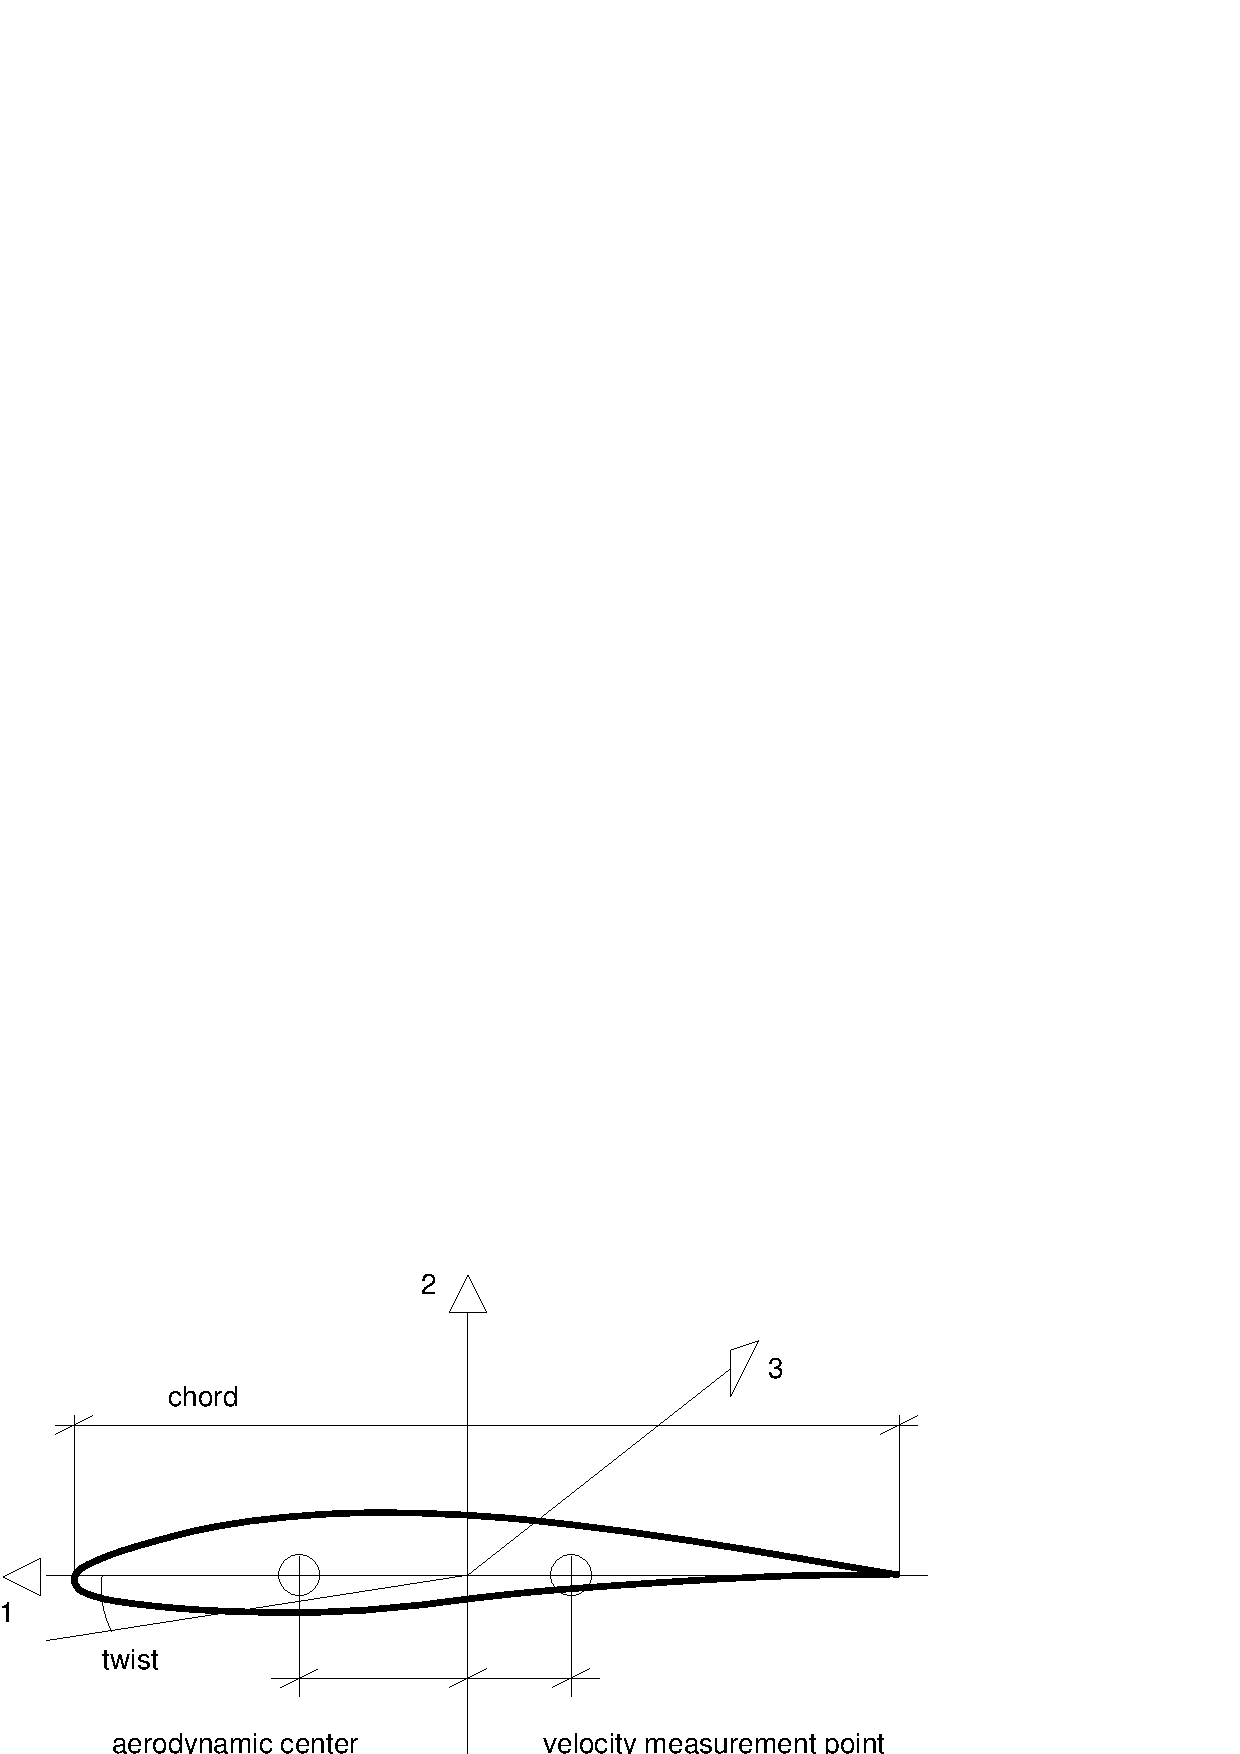
\includegraphics[width=80mm]{airfoil.pdf}
    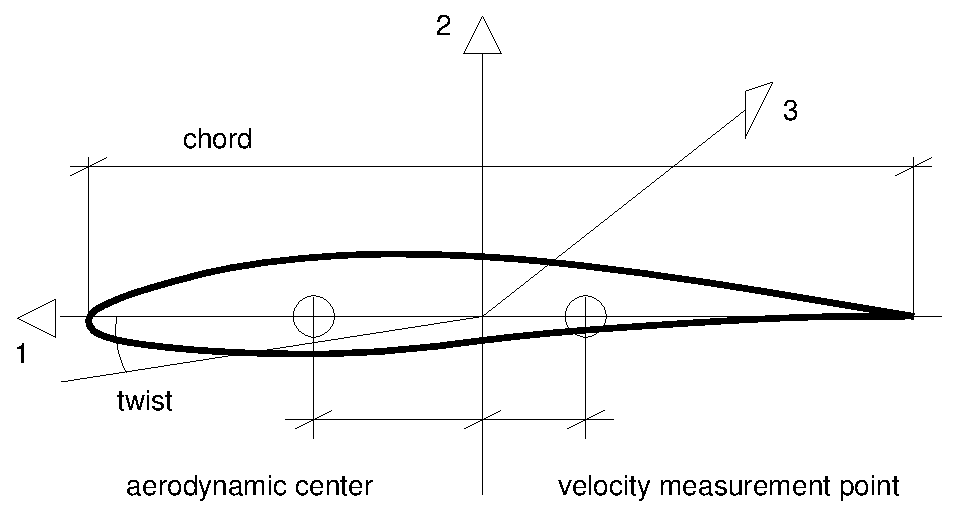
\includegraphics[width=80mm]{airfoil.eps}
  \caption{\em Airfoil Geometry}\label{fig:AIRFOIL}
\end{figure}

The \kw{airfoil\_ data} defaults to a builtin NACA 0012 semianalytical
model (FIXME: the unsteady correction is buggy; use the \kw{c81} 
mode instead).


\subsection{Output}
Aerodynamic elements, both bodies and beams, write their output with file
extension \kw{.aer}; for each time step the required elements are output.
Three different formats are available; the format can be selected only at
compile time, and it must be the same for all the elements. 

\noindent
\emph{Note: eventually it will freeze; if all the output formats will be
maintained, they will be made selectable at run-time.}

\noindent
In any case the label of the element is output first.

\subsubsection{Node}
The format is:
\begin{itemize}
    \item the label of the node
    \item the three components of the force applied to the node
    \item the three components of the couple applied to the node
\end{itemize}
When an \kw{aerodynamic beam} is considered, the output is repeated 
for each node the element is attached to.

\subsubsection{Forces at Gauss points}
The output refers to each Gauss integration point; the format is:
\begin{itemize}
    \item the direction of the wind velocity relative to the element frame
    \item the lift,
    \item the drag,
    \item and the aerodynamic moment per unit length
\end{itemize}
When an \kw{aerodynamic beam} is considered, the output 
is repeated for each portion of beam.

\subsubsection{Coefficients at Gauss points}
The output refers to each Gauss integration point; the format is:
\begin{itemize}
    \item the local incidence
    \item the local yaw angle
    \item the local mach number
    \item the lift,
    \item the drag,
    \item and the aerodynamic coefficient
\end{itemize}
When an \kw{aerodynamic beam} is considered, the output 
is repeated for each portion of the beam.





\section{Aircraft instruments}
\begin{verbatim}
    <card> ::= aircraft instruments
    <arglist> ::= <aircraft_node>
\end{verbatim}
The \kw{<aircraft\_node>} represents the aircraft; it is assumed
that the ``nose'' of the aircraft is towards the positive $x$ direction
of the node, and the ``top'' of the aircraft is towards the positive 
$z$ direction of the node.
The available measures are accessed by defining appropriate 
\kw{parameter} nodes, and by binding the \kw{aircraft instruments} 
element private data to the nodes by means of the \kw{bind} mechanism.
The measures are:
\begin{itemize}
	\item \kw{airspeed}
	\item \kw{groundspeed}
	\item \kw{altitude}
	\item \kw{attitude}
	\item \kw{bank}
	\item \kw{turn}
	\item \kw{slip}
	\item \kw{verticalspeed}
	\item \kw{angleofattack}
\end{itemize}

\noindent
\emph{Note: this element is eXperimental.}




\section{Air Properties Element}
The properties of the airstream are made of the physical properties
of the air plus the description of the airstream velocity direction
and amplitude.
The former can be expressed in different forms, while the latter
are based on three-dimensional vectors which depend on multipliers.
\begin{verbatim}
    <arglist> ::= {
        (drive_caller) <air_density> , (scalar) <sound_speed> 
        | std , { { SI | British }
            [ , temperature deviation , <delta T> ]
            | <p0> , (drive_caller) <rho0> ,
            <T0> , <dT/dz> , <R> , <g0> , <z1> , <z2>
        } [ , reference altitude, <z0> ]
    } , (Vec3_tpl_drive_caller) <air_speed>
\end{verbatim}
The first form consists in the bare input of the air density,
in form of a drive caller, and of the sound celerity, e.g.:
\begin{verbatim}
    air properties: 1.225, 340.,
        1.,0.,0., 150.;
\end{verbatim}
The second form uses standard air properties, both in the
international system (SI) or in British units, possibly
with a temperature deviation and an altitude offset, e.g.:
\begin{verbatim}
    air properties: std, SI, temperature deviation, -55,
        reference altitude, 1000.,
        1.,0.,0., 150.;
\end{verbatim}
where standard properties in SI are used, with a temperature
deviation of -55 K degrees and a reference altitude of 1000 m.
The air properties are computed based on the Z position of the
point where the air properties are requested (plus the optional
altitude offset).
The last possibility requires the user to input all the parameters
required to compute the air properties based on the Z position
of the point where they are requested, namely the reference
pressure \kw{p0}, the reference density \kw{rho0},
the reference temperature \kw{T0}, the initial temperature
gradient \kw{dT/dz}, the gas constant \kw{R}, the
initial gravity acceleration \kw{g0}, the bottom and top
altitudes of the null temperature gradient region \kw{z1} and
\kw{z2}; e.g., for SI units:
\begin{verbatim}
    air properties: std,
        101325.,       /* Pa */
        1.2250,        /* kg/m^3 */
        288.16,        /* K */
        -6.5e-3,       /* K/m */
        287.,          /* J/kgK */
        9.81,          /* m/s^2 */
        11000.,        /* m */
        25000.,        /* m */
        temperature deviation, -55,
        reference altitude, 1000.,
        1.,0.,0., 150.;
\end{verbatim}
The asymptotic air properties are characterized by the drive of the 
air speed, in the global reference frame.





\section{Beam Element}
Currently two beam elements are implemented: a three-node finite volume
element, which has been historically implemented first, which uses
conventional polynomial parabolic interpolation of the nodal displacements
and orientations, and a two-node finite volume element, which has been
recently introduced.
Although this latter element presents some shear-locking, it may be overcome
by correcting the section stiffness matrix in a straightforward form:
\begin{displaymath}
	\hat{K} \ = \ \plbr{F + \frac{L^2}{12}T F T^T}^{-1} ,
\end{displaymath}
where $F=K^{-1}$ is the compliance of the section, and
\begin{displaymath}
	T \ = \ \sqbr{\matr{cc}{
		0 & e_x \times{} \\
		0 & 0
	}}
\end{displaymath}
is the ``arm'' matrix that appears in the differential equilibrium equation
\begin{displaymath}
	\vartheta_{/x} - T^T\vartheta + f \ = \ 0 .
\end{displaymath}
The two-node beam will be reimplemented using a helicoidal interpolation
of the nodal positions and orientations, to reduce the shear-locking effect.

\subsection{Three-node beam element}
The beam element is a three node one-dimensional element.
Each ``node'' is referred to a structural node but can have an arbitrary
offset to allow for more generality in positioning of the structural 
reference lines of the beam.
The ``Finite Volumes'' formulation is used. 
This implies the evaluation of the internal forces at two points 
that are close to the middle point between nodes 1 and 2, 
and between nodes 2 and 3 (at $ 1-1/\sqrt{3} $ from both ends).
So the constitutive properties must be supplied in these points, as well as
the orientation matrices from the material to the global frame (the axial force
is in direction 1).
Any of the allowed 6D constitutive laws can be supplied to define the
constitutive properties.
\begin{verbatim}
    <element_type> ::= beam
    <normal_arglist> ::=
        <node_1> , (Vec3) <relative_offset_1> ,
        <node_2> , (Vec3) <relative_offset_2> ,
        <node_3> , (Vec3) <relative_offset_3> ,
        (OrientationMatrix) <orientation_matrix_section_I> ,
        (ConstitutiveLaw6D) <constitutive_law_section_I> ,
        { same | (OrientationMatrix) <orientation_matrix_section_II> } ,
        { same | (ConstitutiveLaw6D) <constitutive_law_section_II> }
\end{verbatim}
Based on the type of constitutive law, the simple or the viscoelastic beam
element is used.
The two keywords \kw{same} respectively mean that the same orientation 
and the same constitutive law defined for the first point will be used 
for the second point. \\
A piezoelectric actuator beam element is available; an arbitrary
linear piezoelectric actuation matrix is required, together with the labels
of the abstract nodes that represent the input signal tensions, as follows:
\begin{verbatim}
    <normal_arglist> ::=
        <node_1> , (Vec3) <relative_offset_1> ,
        <node_2> , (Vec3) <relative_offset_2> ,
        <node_3> , (Vec3) <relative_offset_3> ,
        (OrientationMatrix) <orientation_matrix_section_I> ,
        (ConstitutiveLaw6D) <constitutive_law_section_I> ,
        (OrientationMatrix) <orientation_matrix_section_II> ,
        (ConstitutiveLaw6D) <constitutive_law_section_II>
        piezoelectric actuator , 
        <electrodes_number> ,
        <abstract_node_label_list> ,
        (Mat6xN) <piezoelectric_matrix_I> ,
        { same | (Mat6xN) <piezoelectric_matrix_II> }
\end{verbatim}
where the \kw{abstract\_node\_label\_list} is the list of the labels of the
abstract nodes that represent the electrodes.

\subsection{Two-node beam element}
\begin{verbatim}
    <element_type> ::= beam2
    <normal_arglist> ::=
        <node_1> , (Vec3) <relative_offset_1> ,
        <node_2> , (Vec3) <relative_offset_2> ,
        (OrientationMatrix) <orientation_matrix_section_I> ,
        (ConstitutiveLaw6D) <constitutive_law_section_I>
        [ , piezoelectric actuator , 
        <electrodes_number> ,
        <abstract_node_label_list> ,
        (Mat6xN) <piezoelectric_matrix_I> ]
\end{verbatim}

\subsection{Output}
The output related to beam elements is contained in a file with extension 
\kw{.act}; for each time step, the output of thre required beams is
considered.
The internal forces and couples are computed from the interpolated strains
along the beam by means of the constitutive law, at the two evaluation
points. 
The format is:
\begin{itemize}
    \item the label of the beam
    \item the three components of the force at the first evaluation point
    \item the three components of the couple at the first evaluation point
    \item the three components of the force at the second evaluation point
    \item the three components of the couple at the second evaluation point    
\end{itemize}



\section{Bind}\label{sec:EL-BIND}
This is not really an element; it is used to instruct a \kw{parameter node}
about which parameter of an element it is bound to.
The \kw{parameter node} must exist, and the binding element, of type 
\kw{element\_type} and label \kw{element\_label}, must have been already 
defined.
The complete syntax is:
\begin{verbatim}
    <arglist> ::= <element_label> , 
                  <element_type> ,
                  <parameter_node_label> , 
                  { <parameter_index> | name , " <parameter_name> " }
\end{verbatim}
Each element makes a number of parameters available for such binding; a
detailed list will be presented in a future release of the input manual.
The value of \kw{parameter\_index} must be legal, i.e.\ between 1 and the
maximum number of parameters made available by the element.
The alternative form, which will become the default, allows more
friendly definition of the binding.
The name of the parameter depends on the element whose property
is being bound.
A complete listing of the parameters that a parameter node 
can be bound to is not available, since most are added based
on developers' needs.
It is advisable that a mechanism for elements to publish 
what parameters they can make available be devised and implemented.

Example: the parameter node \kw{angle} is bound to the rotation
of a revolute hinge.
\begin{verbatim}
    # ... integrator
    begin: control data;
        structural nodes: 2;
        parameter nodes: 2;
        # ... other control data
    end: control data;

    set: integer node1 = 1000;
    set: integer node2 = 2000;
    set integer angle = 5000;

    begin: nodes;
        structural: node1, dynamic, null, eye, null, null;
        structural: node2, dynamic, null, eye, null, null;
        parameter: angle, element;

        # ... other nodes
    end: nodes;

    begin: elements;
        joint: 1, revolute hinge,
            node1, reference, node, null,
                hinge, reference, node, eye,
            node2, reference, node, null,
                hinge, reference, node, eye;
        bind: 1, 1, joint, angle, string, "rx";

        # ... other elements
    end: elements;
\end{verbatim}




\section{Body}
\begin{verbatim}
    <normal_arglist> ::= <node_label> , 
    { 
      (scalar) <mass> , 
      (Vec3)   <relative_center_of_mass> ,
      (Mat3x3) <inertia_matrix>
      [ , inertial , 
          { node | (OrientationMatrix) <orientation_matrix> } ]
    |
      condense, (integer) <num_masses> ,
          (scalar) <mass> , 
          (Vec3)   <relative_center_of_mass> ,
          (Mat3x3) <inertia_matrix> 
          [ , inertial , 
              { node | (OrientationMatrix) <orientation_matrix> } ]
          [ , ... ]
    }
\end{verbatim}
the \kw{inertia\_matrix} is always referred to the center of mass of the
mass that is being added. It can be rotated locally by means of the extra
\kw{orientation\_matrix} supplied after the (optional) keyword \kw{inertial}.
Otherwise, if the keyword \kw{node} is supplied after the keyword 
\kw{inertial}, the inertia matrix is not rotated at all, since it is
assumed to be already in the node reference frame.
If only one mass is defined, the first method should be used. Otherwise,
many masses can be referred to the same element by means of the keyword
\kw{condense}, followed by the number of expected masses \kw{num\_masses}.
The format of each submass is the same as for the single mass input (actually, 
when \kw{condense} is not supplied, \kw{num\_masses} is assumed to be 1).




\section{Bulk Elements}
The \kw{bulk} element is intended as a sort of NASTRAN's \kw{CELAS} card,
that can be used to apply a stiffness term on an arbitrary degree of freedom.
Extensions are planned to different kind of elements.
The syntax of the \kw{bulk} element is:
\begin{verbatim}
    <normal_arglist> ::= <bulk_type> , <bulk_arglist>
\end{verbatim}
At present only the \kw{stiffness spring} type is available.

\subsection{Stiffness spring}
\begin{verbatim}
    <bulk_type> ::= stiffness spring
    <bulk_arglist> ::= (node_dof) <dof> ,
                       (drive_caller) <stiffness_drive>
\end{verbatim}
The equation related to the desired dof of the linked node is added a
contribution based on the value of the desired degree of freedom (even the
derivative can be used) multiplied times the stiffness. \\
{\em Note: this family of elements has been partially superseeded by the
\kw{genel} elements, which allow more generality.}




\section{Couple}
An alias of \kw{force}; see Section~\ref{sec:FORCE}.


\section{Driven Element}
The \kw{driven} type is not an element by itself. It is a wrapper that
masks another element and switches it on and off depending on the (boolean)
value of a drive. It can be used to emulate a variable topology model, where 
some elements simply don't contribute to the residuial or to the jacobian
matrices when their drive has a certain value. Since the drivers can be
arbitrary functions of the time, or other parameters including the value of
any degree of freedom, the driven elements can be ``driven'' in a very
flexible way. Every element can be driven, except those that can be
instantiated once only.
The syntax for a driven element is:
\begin{verbatim}
    <normal_arglist> ::= (drive_caller) <element_driver> ,
        {
            <elem_type> : <elem_label> <elem_normal_arglist> 
        |   
            existing : <elem_type> , <elem_label>
        }
\end{verbatim}
When the first format is used, a normal element is read, instantiated, and
wrapped by the \kw{driven} element wrapper. Note that after the element type,
or after the keyword \kw{existing}, a colon is used as a separator.
This is due for compatibility with the restart module and is not likely 
to be eliminated in the future. 
The label of the element must math that of the driving element given at
the beginning.
When the second format is used, an existing element is sought, and it is
wrapped by a driven element. In this case, no new element is instantiated.
Again the label of the element must match that of the driving element given 
at the beginning. For consistency with the syntax, and for more flexibility,
even when wrapping an existing element it is possible to set at the end the
output flags. This flag will override the previously set one.





\section{Electric Elements}
\kw{electric} elements are those elements that model electric and electronic
devices, dealing with abstract degrees of freedom more than with electric
ones (from the program's point of view they are exactly the same, the
difference is only semantic). The true electric elements, such resistors,
switches and so on, are clessified as \kw{electric bulk} elements.
The syntax for \kw{electric} elements is:
\begin{verbatim}
    <normal_arglist> ::= <electric_type> , <electric_arglist>
\end{verbatim}
The \kw{electric} elements implemented at present are:

\subsection{Accelerometer}
  \begin{verbatim}
    <electric_arglist> ::= <struct_node_label> ,
        <abstract_node_label> ,
        (Vec3) <measure_direction> ,
        (scalar) <omega> ,
        (scalar) <tau> ,
        (scalar) <csi> ,
        (scalar) <kappa>	
  \end{verbatim}
  The label \kw{struct\_node\_label} defines the node whose acceleration 
  is being measured; the label \kw{abstract\_node\_label} defines the
  \kw{abstract node} that will receive the output signal. 
  An \kw{electric node} can be used as well (?).
  The transfer function of the accelerometer is:
  \begin{displaymath}
    \frac{e_0}{a} = \kw{kappa}\frac{\kw{tau} \ s}{
      \plbr{1+\kw{tau} \ s}
      \plbr{1+2 \ \kw{csi}/\kw{omega} \ s+s^2/\kw{omega}^2}
    }
  \end{displaymath}
  where $ e_0 $ is the output signal, $ a $ is the input (the acceleration)
  and $ s $ is the Laplace variable.

\subsection{Discrete control}
  \begin{verbatim}
    <electric_arglist> ::= <num_outputs> , <num_inputs> , <order> ,
        <control_data> , 
        outputs [ , (node_dof) <output_dofs> [ , ... ] ] ,
        inputs [ , (node_dof) <input_dofs> [ , ... ] ] ,
  \end{verbatim}
  The lists of the output and input dofs follows. The input {\tt
  node\_dof}s don't require the \kw{order} field, since they are simply
  used to compute the control forces, and thus identify an equation.
  The \kw{control\_data} has the following syntax:
  \begin{verbatim}  
        <control_data> ::= <control_type> , <control_arglist>
  \end{verbatim}
  At present only a simple form of control is implemented. Other types
  to come are system identification, both recursive and one-shot, and
  adaptive control, with different models and schemes, all based on 
  Generalized Predictive Control (GPC) and Deadbeat Control.
  The \kw{control} syntax is:
  \begin{verbatim}
    <control_data> ::= control , " <control_matrices_file> "
  \end{verbatim}
  where the file \kw{control\_matrices\_file} must contain the matrices
  $ a_c $, $ b_c $ of the control in plain text (as generated by Matlab, for
  instance): \\
  \begin{tabular}{l}
    $ a_{c1} $, \\
    \ldots,     \\
    $ a_{cp} $, \\
    $ b_{c1} $, \\
    \ldots,     \\
    $ b_{cp} $  \\
  \end{tabular} \\
  where $ p $ is the \kw{order} of the controller and the matrices $ a_c $
  have \kw{num\_inputs} rows and \kw{num\_outputs} columns, while the
  matrices $ b_c $ have \kw{num\_inputs} rows and \kw{num\_inputs} columns.





\section{Force}\label{sec:FORCE}
The \kw{force} element has the following syntax:
\begin{verbatim}
  <normal_arglist> ::= <force_type> , <force_arglist>
\end{verbatim}
where \kw{force\_type} can be \kw{abstract} for an abstract force, or 
\kw{conservative} or \kw{follower} for a structural force. The latter types
apply to a \kw{couple} element, which can be structural only.

\subsection{Output}
The output is discussed accordingly to the types of forces. 
The label of the element is output first in all the cases.

\subsection{Abstract force}
\begin{verbatim}
    <force_type> ::= abstract 
    <force_arglist> ::= (node_dof) <dof> ,
                        (drive_caller) <force_magnitude>
\end{verbatim}
the \kw{dof} field is a normal \kw{node\_dof} but no \kw{order} is required
since the \kw{force} simply applies to the equation related to the node,
regardless of the order.

\subsection{Abstract reaction force}
\begin{verbatim}
    <force_type> ::= abstract internal
    <force_arglist> ::= (node_dof) <dof1> ,
                        (node_dof) <dof2> ,
                        (drive_caller) <force_magnitude>
\end{verbatim}
the \kw{dof1} and \kw{dof2} fields are normal \kw{node\_dof}
but no \kw{order} is required since the \kw{force} simply applies
to the equations related to the nodes, regardless of the order, with
opposite magnitudes.

\subsubsection{Output}
The format is:
\begin{itemize}
    \item the label of the element
    \item the label of the abstract node the force is applied to
	(the first node in case of \kw{abstract internal})
    \item the value of the force
\end{itemize}


\subsection{Structural force}
\begin{verbatim}
    <force_type> ::= { conservative | follower } 
    <force_arglist> ::= <node> , 
                        (Vec3) <relative_direction> ,
                        (Vec3) <relative_arm> ,
                        (drive_caller) <force_magnitude>
\end{verbatim}

\subsection{Structural internal force}
\begin{verbatim}
    <force_type> ::= { conservative | follower } internal
    <force_arglist> ::= <node1> , 
                        (Vec3) <relative_direction> ,
                        (Vec3) <relative_arm1> ,
                        <node2> ,
                        (Vec3) <relative_arm2> ,
                        (drive_caller) <force_magnitude>
\end{verbatim}

\subsubsection{Output}
The format is:
\begin{itemize}
    \item the label of the element
    \item the label of the structural node the force is applied to
    \item the value of the force
    \item the three components of the force
    \item the arm of the force, in the global frame (i.e.\ referred
          to point $ \cubr{0,0,0} $)
\end{itemize}


\subsection{Structural couple}
\begin{verbatim}
    <force_type> ::= { conservative | follower } 
    <force_arglist> ::= <node> ,
                        (Vec3) <relative_direction> ,  
                        (drive_caller) <couple_magnitude>
\end{verbatim}

\subsection{Structural internal couple}
\begin{verbatim}
    <force_type> ::= { conservative | follower } internal
    <force_arglist> ::= <node1> ,
                        (Vec3) <relative_direction> ,  
                        <node2> ,
                        (drive_caller) <couple_magnitude>
\end{verbatim}
i.e.\ the arm is not required. 

\subsubsection{Output}
The format is:
\begin{itemize}
    \item the label of the element
    \item the label of the structural node the couple is applied to
    \item the value of the couple
    \item the three components of the couple
\end{itemize}


\noindent
{\em 
Note: by using a \kw{dof} drive, a simple feedback control can be easily
implemented. \\
A more general force element can be written by using a template drive
that contains both the direction and the amplitude. This will be done in the
future. 
}





\section{Genel Element}
\textsc{Genel} is the compact form for \textsc{Gen}eral \textsc{el}ement.
Those elements that cannot in general be classified in a precise way, 
or are just under development and thus are not collected in a class 
of their own until their configuration is stabilized, usually are
classified as \textsc{Genel}.
The syntax of the \textsc{Genel} elements is:
\begin{verbatim}
    <normal_arglist> ::= <genel_type> , <genel_arglist>
\end{verbatim}

\noindent
The output goes in a file with extension \kw{.gen}; only few elements
actually generate output.

\noindent
At present, the \textsc{Genel} class contains very basic general elements
and some special rotorcraft elements.
The latter could be moved to a more specific class in future releases.

\subsection{Special Rotorcraft \textsc{Genel} Elements}
The special \textsc{Genel} elements include the \kw{swashplate}
and the \kw{rotor trim}.

\subsubsection{Swashplate}
The \kw{swashplate} \textsc{Genel} is used to transform the controls 
of a rotor, in terms of collective and fore/aft and lateral cyclic pitch, 
into the elongations of the actuators that actually move the swash plate.
The syntax of the \kw{swashplate} is:
\begin{verbatim}
    <genel_type> ::= swash plate
    <genel_arglist> ::=
        <collective_abstract_node> 
        [ , limits , <min_collective> , <max_collective> ] ,
        <fore/aft_abstract_node> 
        [ , limits , <min_fore/aft> , <max_fore/aft> ] ,
        <lateral_abstract_node> 
        [ , limits , <min_lateral> , <max_lateral> ] ,
        <actuator_1_abstract_node> ,
        <actuator_2_abstract_node> ,
        <actuator_3_abstract_node> 
        [ , <dynamic_coef> , <cyclic_factor> , <collective_factor> ]
\end{verbatim}
The first three abstract nodes will contain the input values (they can be
actuated by means of abstract forces), and the limits on the ``angles'' can
be easily set. 
The last three nodes will contain the values of the stroke of the actuators.
It is assumed that one of the actuators is behind and the others two are in
front of the rotor, numbered clockwise from the top. 
The limits on the actuators will simply force the value of the control
inputs to remain in the boundaries regardless of the input values.
The last three optional parameters are a dynamic coefficient that is used to
add some dynamics to the actuators' stroke, namely the input variables are
applied a sort of \kw{spring stiffness} \kw{bulk} element, while the
actuators' strokes are applied a transfer function of the first order, namely
$ \alpha\dot{x}+x=f $, where $ \alpha=\kw{dynamic\_coef} $ and $ f $ is
the desired stroke, so the smaller is $ \alpha $, the more the behaviour is
static.
The \kw{cyclic\_factor} and the \kw{collective\_factor} parameters are
used to scale the inputs from angles in the desired units to strokes, that
usually are dimensional parameters. The actual strokes are made of the
collective contribution multiplied by \kw{collective\_factor}, and the
cyclic contribution multiplied by \kw{collective\_factor} times 
\kw{cyclic\_factor}.

\subsubsection{Rotor Trim}
The syntax of the \kw{rotor trim} is
\begin{verbatim}
    <genel_type> ::= rotor trim
    <genel_arglist> ::= <rotor_label> ,
        <thrust_node_label> ,
        <longitudinal_moment_node_label> ,
        <lateral_moment_node_label> ,
        (drive_caller) <desired_thrust_coefficient> ,
        (drive_caller) <desired_longitudinal_moment_coefficient> ,
        (drive_caller) <desired_lateral_moment_coefficient> ,
        <rotor_solidity> ,
        <rotor_lock_number> ,
        <rotor_nondimensional_flap_frequency> ,
        <thrust_time_constant> , <moments_time_constant> ,
	<thrust_gain> , <moments_gain>
\end{verbatim}
The \kw{rotor trim} is experimental; it allows to set the controls 
of a generic helicopter, in conjunction with the \kw{swashplate}
element, to asymptotically obtain the desired level of thrust and
moment coefficients.
The corresponding behavior in terms of trim values (flapping angles
and shaft angle) has not been implemented yet.
For details, see \cite{PETERS-TRIM90}.




\subsection{General Purpose Elements}
   
\subsubsection{Clamp}
\begin{verbatim}
    <genel_type> ::= clamp
    <genel_arglist> ::= (node_dof) <clamped_node> ,
                        (drive_caller) <imposed_value>
\end{verbatim}
This element simply forces one arbitrary degree of freedom to assume a value
depending on the drive.

\paragraph{Output}
The format is:
\begin{itemize}
    \item the label of the element
    \item the value of the reaction unknown
\end{itemize}
  
\subsubsection{Distance}
\begin{verbatim}
    <genel_type> ::= distance
    <genel_arglist> ::= (node_dof) <node_1> ,
                        (node_dof) <node_2> ,
                        (drive_caller) <imposed_distance>
\end{verbatim}
This element forces the difference between two arbitrary degrees of freedom
to assume the value dictated by the driver.

\paragraph{Output}
The format is:
\begin{itemize}
    \item the label of the element
    \item the value of the reaction unknown
\end{itemize}
  
  
\subsubsection{Spring}
\begin{verbatim}
    <genel_type> ::= spring
    <genel_arglist> ::= (node_dof) <node_1> ,
                        (node_dof) <node_2> ,
                        (ConstitutiveLaw1D) <const_law>
\end{verbatim}
{\em 
    Note: the constitutive law must be \kw{elastic}, but the \kw{distance}
    genel can apply to arbitrary order degrees of freedom, even between degrees 
    of freedom of different order.
}

\subsubsection{Spring support}
\begin{verbatim}
    <genel_type> ::= spring support
    <genel_arglist> ::= (node_dof) <node> ,                      
                        (ConstitutiveLaw1D) <const_law>
\end{verbatim}
{\em
    Note: the \kw{spring support} must use the \kw{algebraic} value of a 
    \kw{differential} node, but it can use an arbitrary constitutive law,
    i.e.\ an elastic constitutive law for a spring, or a viscous
    constitutive law for a damper, and so on.
}

\subsubsection{Cross spring support}
\begin{verbatim}
    <genel_type> ::= spring support
    <genel_arglist> ::= (node_dof) <row_node> ,                      
                        (node_dof) <col_node> ,                      
                        (ConstitutiveLaw1D) <const_law>
\end{verbatim}
It writes a term depending on the \kw{col\_node} degree of freedom in an
arbitrary manner (given by the \kw{const\_law}) to the 
\kw{row\_node} equation. \\
{\em
    Note: the \kw{cross spring support} must use the \kw{algebraic} value
    of a \kw{differential} node, but can use an arbitrary constitutive law,
    i.e.\ an elastic constitutive law for a spring, or a viscous
    constitutive law for a damper, and so on.
}

\subsubsection{Mass}
\begin{verbatim}
    <genel_type> ::= mass
    <genel_arglist> ::= (node_dof) <node> ,                     
                        (drive_caller) <mass>
\end{verbatim}
{\em
    Note: the mass must use the \kw{algebraic} value of a {\tt
    differential} node. The derivative of the \kw{differential} value of
    the dof is differentiated in a state-space sense, and an inertial driven
    term is applied to the equation related to the dof:
    \begin{eqnarray*}
        m\dot{u} + \ldots & = & f \\
	u - \dot{x} & = & 0
    \end{eqnarray*}
}

\subsubsection{Scalar filter}
\begin{verbatim}
    <genel_type> ::= scalar filter
    <genel_arglist> ::= (node_dof) <output_node> ,
                        (node_dof) <input_node> ,
                        <output_order> [ , <output_coef_list> ] ,
                        <input_order> , <input_coef_list>
                        [ , gain , <gain> ]
\end{verbatim}
This element models a scalar filter of the form
\begin{displaymath}
    A\plbr{s}y = B\plbr{s}u
\end{displaymath}
where $ A $, $ B $ are polynomials of arbitrary order, provided it is
causal, namely the \kw{output\_order} is greater than or equal to 
the \kw{input\_order}.
The polynomial $ A $ is assumed to be monic, so only the coefficients
from 1 to \kw{output\_order} must be input, while all the coefficients 
of polynomial $ B $ are required, i.e.\ from 0 to \kw{input\_order}.
If a gain is supplied, all the coefficients of $ B $ are multiplied by the
gain.

\subsubsection{State space SISO}
\begin{verbatim}
    <genel_type> ::= state space SISO
    <genel_arglist> ::= (node_dof) <output_node> ,
                        (node_dof) <input_node> ,
                        <state_order> ,
                        matrix A , <coefficient_list> ,
                        matrix B , <coefficient_list> ,
                        matrix C , <coefficient_list>
                        [ , matrix D , <coefficient> ]
\end{verbatim}
This element models a scalar (SISO) state space filter of the form
\begin{displaymath}
    \lvvect{ 
        \dot{x} = Ax+Bu \\
	y = Cx+Dx
    }
\end{displaymath}
where $ A $ is a matrix \kw{state\_order}$\times$\kw{state\_order},
$ B $ is a vector \kw{state\_order}$\times$1,
$ C $ is a vector 1$\times$\kw{state\_order},
and $ D $ is scalar, if any.
The matrices are read row-oriented.

\subsubsection{State space MIMO}
\begin{verbatim}
    <genel_type> ::= state space MIMO
    <genel_arglist> ::= <num_outputs> , (node_dof) <output_node_list> ,
                        <num_inputs> , (node_dof) <input_node_list> ,
                        <state_order> ,
                        matrix A , <coefficient_list> ,
                        matrix B , <coefficient_list> ,
                        matrix C , <coefficient_list>
                        [ , matrix D , <coefficient_list> ]
\end{verbatim}
This element models a scalar (SISO) state space filter of the form
\begin{displaymath}
    \lvvect{ 
        \dot{x} = Ax+Bu \\
	y = Cx+Dx
    }
\end{displaymath}
where $ A $ is a matrix \kw{state\_order}$\times$\kw{state\_order},
$ B $ is a matrix \kw{state\_order}$\times$\kw{num\_inputs},
$ C $ is a matrix \kw{num\_outputs}$\times$\kw{state\_order},
and $ D $ is scalar \kw{num\_outputs}$\times$\kw{num\_inputs}.
The matrices are read row-oriented.




\section{Gravity Element}
\begin{verbatim}
    <arglist> ::= (Vec3_tpl_drive_caller) <gravity_acceleration>
\end{verbatim}
the drive of the gravity acceleration, in the global reference frame.




\section{Hydraulic Element}\label{sec:HYDRAULIC-ELEMENT}
{\em 
    Note: under development \\
    Author: Lamberto Puggelli
}
\begin{verbatim}
    <normal_arglist> ::= <hydr_elem_type> , 
                         <hydr_elem_data>
\end{verbatim}
A detailed input description will be given as soon as it is available. \\
\kw{hydraulic\_element\_data} usually contains information about fluid
properties, which are handled by means of an \kw{hydraulic\_fluid}.
This can be directly inserted, following the syntax described in
Section~\ref{sec:HYDRAULIC-FLUID} preceeded by the keyword \kw{fluid}, or a
previously defined fluid can be recalled by using the keyword 
\kw{reference} followed by the label of the desired fluid.

\subsection{Actuator}
\begin{verbatim}
    <hydr_elem_type> ::= actuator ,
    <hydr_elem_data> ::= <node_1> , <node_2> , 
                         <struct_node_1> , (Vec3) <offset_1> ,
                         <struct_node_2> , (Vec3) <offset_2> ,
                         [ direction , (Vec3) <direction> , ]
                         <area_1> ,
                         <area_2> ,
                         <cylinder_length> ,
                         <hydraulic_fluid_properties_1> ,
                         { same | <hydraulic_fluid_properties_2> }
\end{verbatim}

\subsection{Minor Loss}
\begin{verbatim}
    <hydr_elem_type> ::= minor loss ,
    <hydr_elem_data> ::= <node_1> , <node_2> ,
                         <k12> , <k21> , <area> ,
                         <hydraulic_fluid_properties>
\end{verbatim}

\subsection{Control Valve}
\begin{verbatim}
    <hydr_elem_type> ::= control valve ,
    <hydr_elem_data> ::= <node_1> , <node_2> , <node_3> , <node_4>
                         <area> ,
                         [ loss , <loss_factor> , ]
                         (DriveCaller) <state> ,
                         <hydraulic_fluid_properties>
\end{verbatim}
This element represrents a valve that connects
\kw{node\_1} to \kw{node\_2} and \kw{node\_3} to \kw{node\_4}
when \kw{state} is positive and \kw{node\_1} to \kw{node\_3}
and \kw{node\_2} to \kw{node\_4} when \kw{state} is negative,
with area proportional to \kw{area} times the norm of \kw{state}, 
being the latter comprised between $-1$ and $1$.
If \kw{loss\_factor} is defined, it represents the fraction
of area that leaks even when \kw{state} is zero.



\subsection{Dynamic Control Valve}\label{sec:DYNAMIC_CONTROL_VALVE}
\begin{verbatim}
    <hydr_elem_type> ::= dynamic control valve ,
    <hydr_elem_data> ::= <node_1> , <node_2> ,
                         <node_3> , <node_4> ,
                         (DriveCaller) <force> ,
                         <initial_displacement> ,
                         <max_displacement> ,
                         <duct_width> ,
                         [ loss , <loss_factor> , ]
                         <valve_diameter> ,
                         <valve_density> ,
                         <displacement> ,
                         <velocity> ,
                         <acceleration> ,
                         <hydraulic_fluid_properties>
\end{verbatim}
This element represrents a valve that connects
\kw{node\_1} to \kw{node\_2} and \kw{node\_3} to \kw{node\_4}
when the displacement is positive and \kw{node\_1} to \kw{node\_3}
and \kw{node\_2} to \kw{node\_4} when the displacement is negative,
accounting for the dynamics of the valve body.
The control force \kw{force} is applied to the valve, whose 
geometric and structural properties are described by 
\kw{initial\_displacement}, \kw{max\_displacement},
\kw{duct\_width}, \kw{valve\_diameter} and \kw{valve\_density}.
Again the \kw{loss\_factor}, if defined, represents the fraction
of the area that leaks when the displacement is zero.
Finally, \kw{displacement}, \kw{velocity} and \kw{acceleration}
are the penalty coefficients for displacement, valocity and acceleration
when the maximum stroke is reached.




\subsection{Pressure Flow Control Valve}
\begin{verbatim}
    <hydr_elem_type> ::= pressure flow control valve ,
    <hydr_elem_data> ::= <node_1> , <node_2> ,
                         <node_3> , <node_4> ,
                         <node_5> , <node_6> ,
                         (DriveCaller) <force> ,
                         <initial_displacement> ,
                         <max_displacement> ,
                         <duct_width> ,
                         [ loss , <loss_factor> , ]
                         <valve_diameter> ,
                         <valve_density> ,
                         <displacement> ,
                         <velocity> ,
                         <acceleration> ,
                         <hydraulic_fluid_properties>
\end{verbatim}
Same as Dynamic Control Valve (\ref{sec:DYNAMIC_CONTROL_VALVE}),
only the pressures at \kw{node\_5} and \kw{node\_6} are applied
at the sides of the valve body and participate in the force balance.



\section{Joint Element}
Many different joints are available. A first rough classification can be
based on which joints have internal degrees of freedom (the reactions) and
which don't. The latter are flexible joints, that directly add their
stiffness contribution to the dynamic system matrix. From the input point
of view there is no difference between the two classes.
a typical joint entry is made as follows:
\begin{verbatim}
    <normal_arglist> :: = <joint_type> , <joint_arglist>
\end{verbatim}
The output is written to a file with extension \kw{.jnt}.
The output is generally made of a standard part, plus some extra information
depending on the type of joint, which, when available, is described along
with the joint description.
Here the standard part is described:
\begin{itemize}
    \item the label of the joint
    \item the three components of the reaction force in a local reference
    \item the three components of the reaction couple in a local frame
    \item the three components of the reaction force in the global frame
    \item the three components of the reaction couple, rotated into the
          global frame
\end{itemize}
Legal joint types, with relative data, are:


\subsection{Distance}
\begin{verbatim}
    <joint_type> ::= distance 
    <joint_arglist> ::= <node_1> , 
                        [ position , <relative_offset_1> , ]
                        <node_2> ,
                        [ position , <relative_offset_2> , ]
                        { (drive_caller) <distance> | from nodes }
\end{verbatim}

\noindent
{\em 
    Note: the \kw{relative\_offset\_*} are the distances of each end
    of the joint from the relative nodes in the node reference frame \\
    Both the \kw{distance} and the \kw{distance with offset} joints
    allow for null distance, but the transition from null to non-null
    distance is not smooth at all.
} \\
{\em
    Note: in case the keywords \kw{from nodes} are used, a constant drive
    caller is automatically instantiated for the \kw{distance}. 
    Its value is computed from the initial positions of the nodes;
    if defined, the distance between the offsets is considered. 
} \\
{\em
    Note: the \kw{distance with offset} element is deprecated
    in favour of the \kw{distance} with the new syntax, which
    offers the same capabilities.
}
 


\paragraph{Output}
The extra output is:
\begin{itemize}
    \item the three components of the imposed distance in the global frame
    \item the norm of the imposed distance
\end{itemize}



\subsection{Distance with offset}
This element has been deprecated in favour of the \kw{distance}
element, which now supports offsets.  It may be not supported any more
in the future.



\subsection{Clamp}
\begin{verbatim}
    <joint_type> ::= clamp 
    <joint_arglist> ::= <node>
        [ , position ,
            { node | (Vec3) <absolute_position> } ]
        [ , orientation ,
            { node | (OrientationMatrix) <absolute_orientation_matrix> } ]
\end{verbatim}
\emph{Note: the keyword \kw{node} forces the joint to use
the nodal position and reference frame. Otherwise, they must be entered
in the usual way for these entities} \\
\emph{Note: the default value for \kw{position} and \kw{orientation}
are the position and the orientation of the clamped node.}


\subsection{Coincidence}
not implemented yet, use a \kw{spherical hinge} and a \kw{prismatic} 
instead.

\subsection{Spherical hinge}
\begin{verbatim}
    <joint_type> ::= spherical hinge
    <joint_arglist> ::= 
        <node_1> , (Vec3) <relative_offset_1> 
        [ , hinge , 
            (OrientationMatrix) <relative_orientation_matrix_1> ] ,
        <node_2> , (Vec3) <relative_offset_2>
        [ , hinge , 
            (OrientationMatrix) <relative_orientation_matrix_2> ]
\end{verbatim}
{\em
    Note: the orientation matrix is used for output purposes only. 
    A default identity matrix is assumed.
}

\subsection{Pin}
\begin{verbatim}
    <joint_type> ::= pin
    <joint_arglist> ::= <node> , (Vec3) <relative_offset> ,
                                 (Vec3) <absolute_pin_position>
\end{verbatim}
{\em
    Note: this is the dual of the spherical hinge when one node is grounded.
    An alternative way to model a grounded spherical hinge requires the use
    of a static, clamped node.
}

\subsection{Universal hinge}
\begin{verbatim}
    <joint_type> ::= universal hinge
    <joint_arglist> ::= 
        <node_1> , (Vec3) <relative_offset_1> 
        [ , hinge , 
            (OrientationMatrix) <relative_orientation_matrix_1> ] ,
        <node_2> , (Vec3) <relative_offset_2>
        [ , hinge , 
            (OrientationMatrix) <relative_orientation_matrix_2> ]
\end{verbatim}
{\em
    Note: this joint forces the relative direction 3 of node 1 to be always 
    normal to the relative direction 2 of node 2.
}

\subsection{Universal rotation}
A universal joint without position constraints.
\begin{verbatim}
    <joint_type> ::= universal rotation
    <joint_arglist> ::= 
        <node_1>
        [ , hinge , 
            (OrientationMatrix) <relative_orientation_matrix_1> ] ,
        <node_2>
        [ , hinge , 
            (OrientationMatrix) <relative_orientation_matrix_2> ]
\end{verbatim}
{\em
    Note: this joint forces the relative direction 3 of node 1 to be always 
    normal to the relative direction 2 of node 2.
}

\subsection{Universal pin}
\begin{verbatim}
    <joint_type> ::= universal pin
    <joint_arglist> ::= 
        <node> , (Vec3) <relative_offset>
        [ , hinge , 
            (OrientationMatrix) <relative_orientation_matrix> ] ,
        (Vec3) <absolute_pin_position>
        [ , hinge , 
            (OrientationMatrix) <absolute_pin_orientation_matrix> ]
\end{verbatim}
{\em
    Note: this is the dual of the universal hinge when one node is grounded.
}

\subsection{Plane hinge}
This joint has been renamed \kw{revolute hinge}; the old name has been
deprecated and may not be supported in future versions.

\subsection{Revolute hinge}
\begin{verbatim}
    <joint_type> ::= revolute hinge
    <joint_arglist> ::= 
        <node_1> , (Vec3) <relative_offset_1> 
        [ , hinge , 
            (OrientationMatrix) <relative_orientation_matrix_1> ] ,
        <node_2> , (Vec3) <relative_offset_2>
        [ , hinge , 
            (OrientationMatrix) <relative_orientation_matrix_2> ]
\end{verbatim}
{\em
    Note: this joint forces nodes 1 and 2 to rotate only about relative 
    axis 3.
}

\subsection{Revolute rotation}
A revolute joint without position constraints; this joint, in conjunction
with an \kw{inline} joint, should be used to constrain the two nodes
of a hydraulic actuator.
\begin{verbatim}
    <joint_type> ::= revolute rotation
    <joint_arglist> ::= 
        <node_1>
        [ , hinge , 
            (OrientationMatrix) <relative_orientation_matrix_1> ] ,
        <node_2>
        [ , hinge , 
            (OrientationMatrix) <relative_orientation_matrix_2> ]
\end{verbatim}
{\em
    Note: this joint forces nodes 1 and 2 to rotate only about relative 
    axis 3.
}

\subsection{Plane pin}
This joint has been renamed \kw{revolute pin}; the old name has been
deprecated and may not be supported in future versions.

\subsection{Revolute pin}
\begin{verbatim}
    <joint_type> ::= revolute pin
    <joint_arglist> ::= 
        <node> , (Vec3) <relative_offset>
        [ , hinge , 
            (OrientationMatrix) <relative_orientation_matrix> ] ,
        (Vec3) <absolute_pin_position>
        [ , hinge , 
            (OrientationMatrix) <absolute_pin_orientation_matrix> ]
\end{verbatim}
{\em
    Note: this is the dual of the revolute hinge when one node is grounded.
}

\subsection{Axial rotation}
\begin{verbatim}
    <joint_type> ::= axial rotation
    <joint_arglist> ::= 
        <node_1> , (Vec3) <relative_offset_1> 
        [ , hinge , 
            (OrientationMatrix) <relative_orientation_matrix_1> ] ,
        <node_2> , (Vec3) <relative_offset_2>
        [ , hinge , 
            (OrientationMatrix) <relative_orientation_matrix_2> ] ,
        (drive_caller) <angular_velocity>
\end{verbatim}
{\em
    Note: this joint forces nodes 1 and 2 to rotate about relative 
    axis 3 with imposed angular velocity.
}

\subsection{Plane displacement}\label{sec:PLANE_DISPLACEMENT}
This joint allows two nodes to move in the common relative 1--2 plane 
and to rotate about the common relative axis 3.
\begin{verbatim}
    <joint_type> ::= plane displacement
    <joint_arglist> ::= 
        <node_1> , (Vec3) <relative_offset_1> 
        [ , hinge , 
            (OrientationMatrix) <relative_orientation_matrix_1> ] ,
        <node_2> , (Vec3) <relative_offset_2>
        [ , hinge , 
            (OrientationMatrix) <relative_orientation_matrix_2> ]
\end{verbatim}
\emph{Note: this element is temporarily disabled;
combine an \kw{in plane} and a \kw{revolute rotation} joint instead.}

\subsection{Plane displacement pin}
This joint allows a node to move in the relative 1--2 plane 
and to rotate about the relative axis 3 with respect to an absolute point 
and plane.
See also Section~\ref{sec:PLANE_DISPLACEMENT}.
\begin{verbatim}
    <joint_type> ::= plane displacement pin
    <joint_arglist> ::= 
        <node> , (Vec3) <relative_offset>
        [ , hinge , 
            (OrientationMatrix) <relative_orientation_matrix> ] ,
        (Vec3) <absolute_pin_position>
        [ , hinge , 
            (OrientationMatrix) <absolute_pin_orientation_matrix> ]
\end{verbatim}
\emph{Note: this element is temporarily disabled;
combine an \kw{in plane} and a \kw{revolute rotation} joint instead,
using a grounded node.}


\subsection{In plane}
\begin{verbatim}
    <joint_type> ::= in plane
    <joint_arglist> ::= 
        <node_1> , 
        (Vec3) <relative_plane_position> ,
        (Vec3) <relative_normal_direction> ,
        <node_2>
        [ , offset , (Vec3) <relative_offset>]
\end{verbatim}
{\em
    Note: to make an in-line joint, use two in-plane joints, with the
    planes that intersect along the desired line. \\
    Note: a \kw{inline} element has been added, which automates the above
    reported procedure.
}

\subsection{In line}
\begin{verbatim}
    <joint_type> ::= in line
    <joint_arglist> ::= 
        <node_1> , 
        (Vec3) <relative_line_position> ,
        (Mat3x3) <relative_orientation> ,
        <node_2>
        [ , offset , (Vec3) <relative_offset>]
\end{verbatim}
{\em 
    Note: the \kw{in line} joint supersedes the former note; the orientation
    assumes the sliding line is in direction 3.
}

\subsection{Rod}
\begin{verbatim}
    <joint_type> ::= rod 
    <joint_arglist> ::= <node_1> , <node_2> , 
        (scalar) { <rod_length> | from nodes }
        [ , offset , (Vec3) <relative_offset_1> , 
                     (Vec3) <relative_offset_2> ] ,
        (ConstitutiveLaw1D) <const_law>
\end{verbatim}
The constitutive law \kw{<const\_law>} is used in form 
of rod axial stiffness $EA$, i.e., for a linear constitutive law:
\begin{displaymath}
	F = EA \frac{l - l_0}{l_0}
\end{displaymath}
and in general
\begin{displaymath}
	F = F\plbr{\frac{l - l_0}{l_0}, \frac{\dot{l}}{l_0}}
\end{displaymath}
where $l_0=\kw{<rod\_length>}$.
For further details on the constitutive laws, 
see Section~\ref{sec:CONSTITUTIVE-LAWS}.
See also \kw{rod with offset} in Section~\ref{sec:RD-WITH-OFFSET}.

\subsection{Rod with offset}\label{sec:RD-WITH-OFFSET}.
\begin{verbatim}
    <joint_type> ::= rod with offset
    <joint_arglist> ::= <node_1> , (Vec3) <relative_offset_1>
                        <node_2> , (Vec3) <relative_offset_2>
        (scalar) { <rod_length> | from nodes } ,
        (ConstitutiveLaw1D) <const_law>
\end{verbatim}
Analogous to \kw{rod} with the optional arg \kw{offset}.

\subsection{Deformable hinge}
\begin{verbatim}
    <joint_type> ::= deformable hinge
    <joint_arglist> ::= 
        <node_1>
        [ , hinge , (OrientationMatrix) <relative_orientation_matrix_1> ] ,
        <node_2> 
        [ , hinge , (OrientationMatrix) <relative_orientation_matrix_2> ] ,
        (ConstitutiveLaw3D) <const_law>
\end{verbatim}
\emph{Note: this hinge constrains the orientations only.
    It should be used in conjunction with a spherical hinge or any kind of
    joint that constrains the displacements too.}

\subsection{Deformable displacement hinge}
\begin{verbatim}
    <joint_type> ::= deformable displacement hinge
    <joint_arglist> ::= 
        <node_1> , (Vec3) <relative_offset_1>
        [ , hinge , (OrientationMatrix) <relative_orientation_matrix_1> ] ,
        <node_2> , (Vec3) <relative_offset_2>
        [ , hinge , (OrientationMatrix) <relative_orientation_matrix_2> ] ,
        (ConstitutiveLaw3D) <const_law>
\end{verbatim}

\subsection{Linear velocity}
\begin{verbatim}
    <joint_type> ::= linear velocity
    <joint_arglist> ::= <node> , (Vec3) <relative_direction> , 
                        (drive_caller) <velocity>
\end{verbatim}

\subsection{Angular velocity}
\begin{verbatim}
    <joint_type> ::= angular velocity
    <joint_arglist> ::= <node> , (Vec3) <relative_direction> , 
                        (drive_caller) <velocity>
\end{verbatim}

\subsection{Linear acceleration}
\begin{verbatim}
    <joint_type> ::= linear acceleration
    <joint_arglist> ::= <node> , (Vec3) <relative_direction> , 
                        (drive_caller) <acceleration>
\end{verbatim}

\subsection{Angular acceleration}
\begin{verbatim}
    <joint_type> ::= angular acceleration
    <joint_arglist> ::= <node> , (Vec3) <relative_direction> , 
                        (drive_caller) <acceleration>
\end{verbatim}

\subsection{Prismatic}
\begin{verbatim}
    <joint_type> ::= prismatic
    <joint_arglist> ::= 
        <node_1>
        [ , hinge , (OrientationMatrix) <relative_orientation_matrix_1> ] ,
        <node_2> 
        [ , hinge , (OrientationMatrix) <relative_orientation_matrix_2> ] ,    
\end{verbatim}

\subsection{Drive hinge}
\begin{verbatim}
    <joint_type> ::= drive hinge
    <joint_arglist> ::= 
        <node_1>
        [ , hinge , (OrientationMatrix) <relative_orientation_matrix_1> ] ,
        <node_2> 
        [ , hinge , (OrientationMatrix) <relative_orientation_matrix_2> ] ,
        (Vec3_tpl_drive_caller) <hinge_orientation>
\end{verbatim}
\emph{Note: this element is eXperimental; now it is more reliable, 
but it is limited to $\nrbr{\tt <hinge\_orientation>} < \pi$}.

\subsection{Kinematic}
This joint will eventually evolve into a connection with external programs
that impose the entire motion of a node; at present, you can use it
by directly writing code in files \verb;mbdyn/struct/kin.cc; and
\verb;mbdyn/struct/kin.h; that implement the motion you wish to impose.
\begin{verbatim}
    <joint_type> ::= kinematic
    <joint_arglist> ::= 
        <node_1> ,
        (drive_caller) <input>
\end{verbatim}
\emph{Note: this element is eXperimental.}
 
\subsection{Modal}\label{ELEMS-JOINT-MODAL}
\emph{Note: under development \\
    Author: Felice Felippone;
    Initial review: Giuseppe Quaranta;
    Current review: Pierangelo Masarati.}

\begin{verbatim}
    <joint_type> ::= modal
    <joint_arglist> ::=
        { <reference_modal_node> | clamped
            [ , position , (Vec3)<absolute_position> ]
            [ , orientation , (Mat3x3)<absolute_orientation> ] } ,
        <mode_number> ,
        [ , list, <mode> [ , ... ] ]
        <fem_node_number> 
        [ , no damping 
            | proportional damping , <damping_coef>
            | diag damping , 
                <mode_index> , <mode_damping_coef> 
                [ , ... ] 
        ] , " <fem_data_file> " ,
        [ , origin node , <origin_node> ]
        <interface_nodes_number> ,
            <fem_node_label> ,
                <multibody_label> , (Vec3)<offset_of_FEM_node>
            [ , ... ] ,
        " <output_file_name> "
\end{verbatim}
The \kw{reference\_modal\_node} is a special dynamic structural node 
that is required to handle the rigid body motion of the modal joint.
Its input is completely analogous to that of the \kw{dynamic} structural
nodes, see Section~\ref{sec:NODE-STRUCT}, only the keyword \kw{dynamic} 
must be replaced by \kw{modal}.

\noindent
If no rigid body dynamics is required, e.g.\ if the modal element
is clamped, the \kw{clamped} option can be used, which allows
to set the optional \kw{absolute\_position} 
and \kw{absolute\_orientation}; they default to zero and identity.

\noindent
The mode count in \kw{mode\_number} is not required to match
the number of modes listed in the FEM data file; if a lower number
is given, only the first \kw{mode\_number} modes are used;
moreover, a list of active modes can be given, to use non-consecutive
modes; e.g., to use modes 1, 2, 3 and 6 of a set of 10 modes, use:
\begin{verbatim}
	4, list, 1, 2, 3, 6
\end{verbatim}

\noindent
The origin of the FEM grid is placed either in the position and orientation 
of the modal node, or in the absolute position and orientation 
in case the modal element is clamped, unless the \kw{origin node} 
optional keyword is used.
It defines what FEM node corresponds to the \kw{modal} node,
or what node lies in the absolute position and orientation
for a clamped modal element.

\noindent
The list of matchings between FEM and multibody nodes needs
special care.
The \kw{offset\_of\_FEM\_node} field contains the distance
of the FEM node from the respective multibody node.

\noindent
The \kw{fem\_data\_file} can be generated by NASTRAN, using
the ALTER cards provided in directory \kw{etc/modal.d/} 
of the distribution.
In detail:
\begin{enumerate}
\item the file \kw{MBDyn\_NASTRAN\_alter\_1.nas} contains
	ALTER definitions for static solutions; appropriate
	loading subcases for each solution must be provided
	in the case control and in the bulk data sections
	of the input file;

	\emph{FIXME: I don't know how to use static shapes only}.

\item the file \kw{MBDyn\_NASTRAN\_alter\_2.nas} contains
	ALTER definitions for eigenanalysis solutions;
	an appropriate eigenanalysis method, with the related
	data card must be provided in the case control 
	and in the bulk data sections of the input file;

	\emph{FIXME: I don't know how to use this together
		with static shapes; I only get the normal mode shapes,
		even if the matrices are complete}.

\item the file \kw{MBDyn\_NASTRAN\_alter\_3.nas} contains
	ALTER definitions for eigenanalysis solutions;
	an appropriate eigenanalysis method, with the related
	data card must be provided in the case control 
	and in the bulk data sections of the input file;

	\emph{Note: this works; see} \kw{tests/modal/beam.README}.

\end{enumerate}
The static solution of case (1: \kw{SOL 101}) and the eigensolution
of case (2: \kw{SOL 103}) need to be performed in sequence; 
if only the eigensolution is to be used, the ALTER file 
of case (3: \kw{SOL 103}) must be used.
The static solution of case (1) generates a binary file \kw{mbdyn.stm};
the eigensolutions of cases (2--3) generate two binary files, 
\kw{mbdyn.mat} and \kw{mbdyn.tab}; then, the tool \kw{utils/femgen} 
must be executed, which transforms the binary files into 
the \kw{fem\_data\_file}; the file name is requested as terminal input.

\noindent
It is strongly recommended that constrained modal analysis
be used for otherwise free bodies, with the statically 
determined constraint consisting of clamping the FEM node 
that will coincide with \kw{reference\_modal\_node}, and using
the \kw{origin node} to make that point the origin of the FEM frame.

\noindent
About reference frames ...

\noindent
The format of the \kw{fem\_data\_file} is relatively straightforward;
each data block is commented.
In detail, initial modal displacements and velocities can be added,
if required, by manually editing the file; however this practice
is discouraged.



\subsection{Beam slider}
This joint implements a slider, e.g.\ it constrains a structural node 
on a string of three-node beams, as discussed in \cite{SLIDER-AIDAA-2003}.
\begin{verbatim}
    <joint_type> ::= kinematic
    <joint_arglist> ::=
        <slider_node> ,
        (Vec3) <relative_offset> ,
        [ hinge , (OrientationMatrix) <relative_or_mat> ] ,
        [ type , { spherical | classic | spline } , ]
        <beam_number> ,
            <3_node_beam> ,
                { same | (Vec3) <first_node_offset> } ,
    [ hinge , { same | (OrientationMatrix) <first_node_or_mat> ] , }
                (Vec3) <mid_node_offset> ,
    [ hinge , (OrientationMatrix) <mid_node_or_mat> ] ,
                (Vec3) <end_node_offset> ,
    [ hinge , (OrientationMatrix) <end_node_or_mat> ] ,
                [ ... ]
        [ , initial beam , <initial_beam> ]
        [ , initial node, <initial_node> ]
        [ , smearing, <smearing_factor> ]
\end{verbatim}
There are three types of slider:
\begin{itemize}
	\item the \kw{spherical} slider does not constrain
	the orientation of the node;
	\item the \kw{classical} slider does allow rotation
	only about the sliding line;
	\item the \kw{spline} slider constrain the orientation
	of the node.
\end{itemize}
For each node of each beam element, the offset and the orientation
of the slider can be defined; except for the first element, the
offset and the orientation of the first node can be specified using
the keyword \kw{same}, which causes the node to take the same
value of the last node of the previous beam.
The \kw{initial\_beam} and \kw{initial\_node} indices
serve as hints to set the initial contact point of the sliding node.
The \kw{smearing\_factor} determines the (nondimensional) extension
of the interference segment when the node passes from one segment
to another. % \cite{SLIDER}.

\section{Loadable Element}
The \kw{loadable} element is a wrapper for a user-defined element that is
comipled in a separated module and linked run-time.
The module should provide a comprehensive set of functions with a specified
API; default functions are available if no special features are required.
Implementation of modules can be very easy, but a deep knowledge of the
internals of the code is required if special tasks are required. 
There are virtually no limits on what a loadable element can do.
The syntax is simply:
\begin{verbatim}
    <normal_arglist> ::= " <module_name> "
                         [ , name, " <calls> " ] 
                         [ , <module_data> ]
\end{verbatim}
where \kw{module\_name} is the name of the module file; as soon as the file
is checked and the binding of the structure with function bindings 
succeeded, a function called \kw{read} is invoked, and passed the input
stream.
This function is in charge of reading \kw{module\_data} following the
general syntax of the input file.

It is advisable that the function \kw{read} prints some help message
when the first field of \kw{module\_data} is the keyword \kw{help}.
All the helpers and the high-level structures are available, such as
drivers, constitutive laws, reference frames.
Refer to each module for a description (if available) of the features and of
the input/output format.
\kw{module\_name} should be a full path to the module function.
If the name starts with a slash ``/'', the full path name is used.
Otherwise the module is searched in the colon-separated list of directories 
contained in the environment variable \kw{LD\_LIBRARY}, then among the
libraries listed in \kw{/etc/ld.so.cache}, and finally in
\kw{/usr/lib} and in \kw{/lib} (see \kw{dlopen(3)}).
At last, it is searched in the current directory, and the extension
\kw{.so} is added if missing.
The string \kw{<calls>} represents the name of the structure that contains
the bindings to the functions.
The default is \kw{calls}.

\noindent
Refer to \kw{\$(BASE)/mbdyn/base/loadable.h} for a description of the
functions that are allowed.
An example module is given in directory
\begin{verbatim}
    $(BASE)/modules/module-template/
\end{verbatim}
which can be used as a starting point for building a custom module.
% An analogous C/FORTRAN style interface is being planned, at the cost of
% possibly losing some of the fancy C++ features made available by the code.
The \kw{loadable element} interface allows to link modules in different
languages, e.g.\ C or FORTRAN77; simply use \kw{module-template}
as a guideline to providing callbacks to the \kw{loadable element}
interface and to collect required info from the main program
(e.g.\ node positions, equation indices and everything else that is
required for appropriate connection), then call the functions that
actually do the work in other languages from inside the callbacks.
Note that, in general, to call external functions from C++ one needs
to declare them as
\begin{verbatim}
    #include <sys/types.h>
    extern "C" {
        int a_C_function(int arg, double darg);
        int a_F77_subroutine(int32_t *iarg, double *darg);
    }
\end{verbatim}
The same applies to FORTRAN 77 functions; only, the naming convention
usually is compiler dependent; some compilers turn all the names to 
uppercase or lowercase (remember that FORTRAN 77 is case insensitive);
other compilers add undercores at the beginning or at the end of the
names.
Check what is the behavior of your compiler, by compiling a simple 
program with your favourite FORTRAN 77 compiler, then looking at it
with the utility \kw{nm(1)}, which will show how the symbols are represented 
internally.

\noindent
For instance, the code
\begin{verbatim}
C This is a compiler test
      SUBROUTINE F77SUB(I, D)
      INTEGER*4 I
      REAL*8 D(*)

      D(I) = 0.0

      END
\end{verbatim}
when compiled with \kw{g77(1)} on a Linux system, yields:
\begin{verbatim}
[masarati@mbdyn manual]$ g77 -c f77sub.f
[masarati@mbdyn manual]$ nm f77sub.o
00000000 T f77sub_
\end{verbatim}
That is, \kw{g77(1)} lowercases all symbols, and adds a trailing 
underscore.
Macros to automatically detect and take care of this behavior 
will be added.


\noindent
To compile loadable modules, one needs to configure
the package as follows:
\begin{verbatim}
    ./configure --with-module=<module_name>
\end{verbatim}
where \kw{module\_name} is the name of the directory the module
is placed in with the \kw{module-} part stripped; e.g.\ to compile
the tire module that resides in \kw{\$(BASE)/modules/module-wheel2} 
one must type
\begin{verbatim}
    ./configure --with-module=wheel2
\end{verbatim}
Multiple modules can be compiled by typing the list of the names
separated by blanks.
The modules need to resolve some of the symbols that are in the
main executable; until a full working libtool support is implemented,
this must be done by hand.
For the \kw{g++(1)} compiler one requires the switch \kw{-rdynamic} 
to be added to the loader flags, e.g.
\begin{verbatim}
    LDFLAGS="-rdynamic" ./configure --with-module=<module_name>
\end{verbatim}
on \kw{sh(1)} and compatible shells like \kw{bash(1)}, or
\begin{verbatim}
    env LDFLAGS="-rdynamic" ./configure --with-module=<module_name>
\end{verbatim}
on \kw{csh(1)} and compatible shells.





\section{Output Elements}

\subsection{RTAI output}\label{sec:RTAI_out}
This is a special element which takes care of sending generic output
to external processes by means of RTAI mailboxes during real-time 
simulations.
This topic is under development, so expect frequent changes, and
please do not count too much on backward compatibility.
The syntax is:
\begin{verbatim}
    <normal_arglist> ::=
        name , " <mailbox_name> " ,
        create , { yes | no } ,
        [ host , " <host_name> " , ]
        <channel_number> ,
            (node_dof) <output_dof>
            [ , ... ]
\end{verbatim}
where
\begin{itemize}
\item \kw{<mailbox\_name>} is the name of the RTAI mailbox where 
the output is written  (a unique string not longer than six chars);
\item the \kw{create} keyword determines whether the mailbox
must be created or looked-up as already existing on the system;
\item \kw{<host\_name} is the name or the IP of the remote host where
the mailbox resides; note that if this field is given, \kw{create} must
be set to \kw{no} and the mailbox must be already defined
on the remote host;
\item the number of channels \kw{<channel\_number>} that are written
determines how many \kw{node\_dof} entries must be read.
They must be valid scalar dof entries, which can be connected
in many ways to nodal degrees of freedom or to element private data.
\end{itemize}

\emph{Note: at present, these elements require that the simulation
be run in real-time mode (see Section~\ref{sec:REAL-TIME});
future development will allow to emulate the use of these elements
also when the simulation is not run in real-time, e.g.\ for modeling
or model debugging purposes.}






\subsection{Stream output}\label{sec:STREAM_OUTPUT}
This is a special element which takes care of sending generic output
to external processes by means of RTAI mailboxes during real-time 
simulations.
This topic is under development, so expect frequent changes, and
please do not count too much on backward compatibility.
The syntax is:
\begin{verbatim}
    <normal_arglist> ::= stream output
        name , " <mailbox_name> " ,
        create , { yes | no } ,
        [ { local , " <socket_name> " , |
            [ port , <port_number> , ]
            [ host , " <host_name> " , ] } ]
        <channel_number> ,
            (node_dof) <output_dof>
            [ , ... ]
\end{verbatim}
The stream output allows MBDyn to send streamed outputs 
to remote processes both during regular simulations and during 
real-time simulations under RTAI.
If the simulation is run in real-time, it uses RTAI mailboxes, 
otherwise regular UNIX sockets are used, either in the \kw{local} or 
in the \kw{internet} namespace.

This output element type is intended to allow the development 
of real-time models by running regular simulations for the purpose 
of debugging the model and the control process without the overhead 
and the potential problems of running in real-time.
Then the same model can be run in real-time without changing the details
of the communication with the controller process.

\paragraph{Non real-time simulation}
During non real-time simulations, streams operate in blocking mode.
The meaning of the parameters is:
\begin{itemize}
\item \kw{<name>} indicates the name the stream
will be known as; it is limited to 6 characters, and mostly useless;
\item the instruction \kw{create} determines whether the socket will be
created or looked for by MBDyn;
\item the keyword \kw{local} indicates that a socket 
in the local namespace will be used; if \kw{create} is set to \kw{yes},
the socket is created, otherwise it must exist.
\item either of the keywords \kw{port} or \kw{host} indicate that a socket
in the internet namespace will be used;
if \kw{create} is set to \kw{yes}, \kw{<host\_name>} indicates 
the host that is allowed to connect to the socket; it defaults 
to any host (\kw{0.0.0.0}); if \kw{create} is set to \kw{no},
\kw{<host\_name>} indicates what host to connect to; the default 
is localhost (\kw{127.0.0.1}); the default port is \kw{5500};
\end{itemize}
If no socket type is specified, i.e.\ none of the \kw{local}, \kw{port} 
and \kw{host} keywords are given, a socket is opened by default 
in the internet namespace with the default IP and port; the \kw{create}
keyword is mandatory.

\paragraph{Real-time simulation}
During real-time simulations, streams wrap non-blocking RTAI mailboxes.
The meaning of the parameters is:
\begin{itemize}
\item the parameter \kw{<name>} indicates the name the stream
will be known as in RTAI's resource namespace; it is limited to 6 characters;
\item the instruction \kw{create} determines whether the mailbox will be
created or looked for by MBDyn;
\item the keyword \kw{local} is ignored;
\item the keyword \kw{host} indicates that a mailbox on a remote host 
will be used; it is useless when \kw{create} is set to \kw{yes}, because
RTAI does not provide the possibility to create remote resources;
if none is given, a local mailbox is assumed;
\item the keyword \kw{port} is ignored.
\end{itemize}

The number of channels \kw{<channel\_number>} that are written
determines how many \kw{node\_dof} entries must be read.
They must be valid scalar dof entries, which can be connected
in many ways to nodal degrees of freedom or to element private data.






\section{Rotor Element}
The \kw{rotor} element is used to associate the aerodynamic elements that
model the blades of a rotor when some inflow related computations are
required. By means of different inflow models, and by means of the
aerodynamic load contributions supplied by the aerodynamic elements, the
rotor element is able to compute the induced velocity at an arbitrary point on
the rotor disk. This velocity term on turn is used by the aerodynamic
elements to determine a better estimate of the boundary conditions.
The syntax of the \kw{rotor} element is:
\begin{verbatim}
    <normal_arglist> ::= <craft_node> ,
            [ hinge , (Mat3x3)<rotor_orientation> , ]
        <rotor_node> ,
        induced velocity , <induced_velocity_model>
\end{verbatim}
The optional \kw{rotor\_orientation} is required when axis 3 
of the \kw{craft\_node} is not aligned with the rotor axis; axis 3
of the \kw{rotor\_node} must be aligned with the rotor axis.

\emph{Note: after the keyword \kw{induced velocity} there used to be
a colon is used as separator.
This changed for uniformity with the rest of the syntax.
No backwards compatibility is provided, so users are urged to update
their models.
A warning is issued.
}

\noindent
There are five models of induced velocity. 
The first is no induced velocity; the syntax is:
\begin{verbatim}
    <induced_velocity_model> ::= no
\end{verbatim}
There is no argument list. This element doesn't compute any induced
velocity, but still computes the rotor traction for output purposes,
if output is required.
The others have a fairly common syntax.  The first three are
\kw{uniform}, \kw{glauert} and \kw{mangler} induced velocity
models:
\begin{verbatim}
    <induced_velocity_model> ::= { uniform | glauert | mangler } , 
        <reference_omega> , <reference_radius> 
        [ , ground , <ground_node> ]
        [ , delay , (drive_caller) <memory_factor> ]
        [ , max iterations , <max_iterations> ]
        [ , tolerance , <tolerance> ]
        [ , eta , <eta> ]
        [ , correction , <hover_correction_factor> ,
            <ff_correction_factor> ]
\end{verbatim}
the \kw{reference\_omega} field is used to decide whether to inhibit
or not the induced velocity computation if the rotor speed is very low;
the \kw{reference\_radius} field is used in the adimensionalization
of the rotor related parameters. \\
The \kw{memory\_factor}, the \kw{hover\_correction\_factor} 
and the \kw{ff\_correction\_factor} (forward flight) are
used to correct the nominal induced velocity, according to the formula
%\begin{eqnarray*}
%	U_{effective} & = &
%	\plbr{1 - \kw{memory\_factor}} 
%		\kw{correction\_factor} \ U_{nominal} \\
%	& & \mbox{} + \kw{memory\_factor} \ U_{previous}
%\end{eqnarray*}
\begin{eqnarray*}
	U_{effective} & = &
	\plbr{1 - \mathtt{<memory\_factor>}} 
		U_{nominal} \\
	& & \mbox{} + \mathtt{<memory\_factor>} \ U_{previous}
\end{eqnarray*}
with
\begin{displaymath}
	U_{nominal} = \frac{T}{2 \rho A V_{tip} \sqrt{
		\cfrac{\lambda^2}{\mathtt{<hover\_correction\_factor>}^4}
		+ \cfrac{\mu^2}{\mathtt{<ff\_correction\_factor>}^2}
	}}
\end{displaymath}
The \kw{memory\_factor} parameter is used to
combine the current reference induced velocity with the induced velocity
at the previous step; no delay means there is no memory of the previous value 
(\emph{Note: for historical reasons, the keyword \kw{weight}
can be used instead of \kw{delay}}). \\
The \kw{memory\_factor} parameter defaults to 0; 
the \kw{hover\_correction\_factor} 
and the \kw{ff\_correction\_factor} parameters default to 1. \\
The \kw{max\_iterations}, the \kw{tolerance} 
and the \kw{eta} parameters refer to the iteration cycle 
that is performed to compute the nominal induced velocity; 
after \kw{max\_iterations}, or when the absolute value 
of the difference between two iterations of the nominal induced 
velocity is less than \kw{tolerance}, the cycle breaks.
Only a fraction \kw{eta} of the difference between two
interations of the nominal induced velocity is actually
used; \kw{eta} defaults to one.
The default is to make only one iteration, which is backward-compatible
with the original behavior.
\emph{
	Note: the syntax of the correction factor input changed
	from MBDyn 1.1 to MBDyn 1.2, where two different factors,
	according to conventional models (e.g.\ CAMRAD/JA), have
	been considered instead of one.
	No backward compatibility has been implemented because 
	this is a very specialistic parameter and it was introduced 
	very recently.
}

\noindent
The last one uses a dynamic inflow model, based on \cite{PITT},
with inflow states.
The syntax is:
\begin{verbatim}
    <induced_velocity_model> ::= dynamic inflow , 
        <reference_omega> , 
        <reference_radius> 
        [ , ground , <ground_node> ]
        [ , initial value , <const_vel> ,
            <cosine_vel> ,
            <sine_vel> ]
        [ , max iterations , <max_iterations> ]
        [ , tolerance , <tolerance> ]
        [ , eta , <eta> ]
        [ , correction , <hover_correction_factor> ,
            <ff_correction_factor> ]
\end{verbatim}
Most of the entries are the same as for the previous models;
the \kw{delay} optional entry is missing, while the three states, 
corresponding to average, fore-aft and lateral inflow,
can be explicitly initialized by means of the optional 
entry \kw{initial value}.



\section{Miscellaneous}
This section lists some extra cards that do not correspond to any
specific simulation entity, but rather alter the behavior 
of existing entries or cause special operations to be undertaken
during model input.

\subsection{Inertia}
This card causes the equivalent inertia properties of a subset
of elements to be generated.
\begin{verbatim}
    <card> ::= inertia : <label>
        [ , name , " <inertia_name> " ]
        [ , position , (Vec3)<reference_position> ]
        [ , orientation , (Mat3x3)<reference_orientation> ]
        , <type_subset> [ , ... ] ;
        <type_subset> ::= <type> , { all | <label_list> }
        <label_list> ::= <label> [ , <label_list> ]
\end{verbatim}
where \kw{type} currently can only be \kw{body}, although more elements
associated to inertia might participate in the future.
All elements whose labels are listed must exist, and duplicates
are detected and considered errors.
The keyword \kw{all} causes all the elements of type \kw{type} 
to be included in the list.
As a result, each \kw{inertia} entry is logged in the \kw{.log} file
in a self explanatory form, referred both to the \kw{global} 
reference frame and to the reference frame n \kw{reference\_position}
oriented as \kw{reference\_orientation}.



\subsection{Output}
There is an extra card that is used to modify the output behaviour of 
elements, analogous to that of the nodes:
\begin{verbatim}
    <card> ::= output : <elem_type> , <elem_list> ;
    <elem_list> ::= <elem_label>  [ , <elem_list> ]
\end{verbatim}
\kw{elem\_type} is a valid element type that can be read 
as card name in the \kw{elements} block.
module.





